\documentclass{standalone}
\usepackage{tikz}
\usepackage{amsthm, amssymb,latexsym}
\usepackage{bbm}
\usepackage{pgfplots}
\usepackage{mathtools}

%\usetikzlibrary{...}% tikz package already loaded by 'tikz' option

\begin{document}
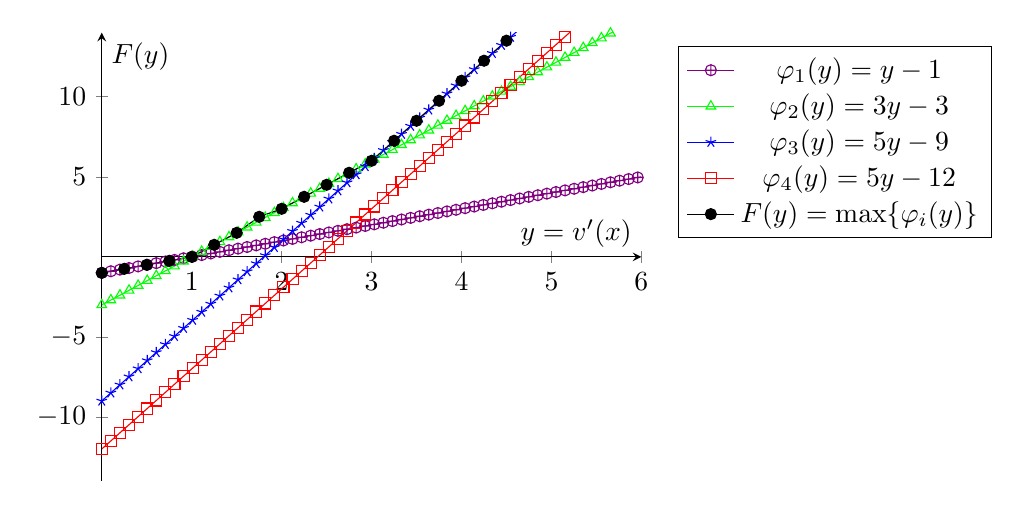
\begin{tikzpicture}
\begin{axis}[
    axis lines = middle,
    xlabel = {$y=v'(x)$},
    ylabel = {$F(y)$},
    legend style={at={(1.65,0.97)},
    anchor=north east},
    xmin=0, xmax=6,
    ymin=-14, ymax=14,
]
\centering
\addplot [
    domain=0:10,
    samples=100,
    color=violet,
    mark=oplus,
    ]
    {x-1};
\addlegendentry{$\varphi_1(y)=y-1$}

 \addplot [
    domain=0:10,
    samples=100,
color=green,
    mark=triangle
        ]
    {(3*x -3};
\addlegendentry{$\varphi_2(y)=3y -3$}


\addplot [
    domain=0:10,
    samples=100,
    color=blue,
    mark=star,
    ]
    { 5*x -9};
\addlegendentry{$\varphi_3(y)=5y -9$}


\addplot [
   domain=0:10,
    samples=100,
    color=red,
    mark=square,
]
{5*x - 12};
\addlegendentry{$\varphi_4(y)=5y - 12$}


\addplot [
     color=black,
     mark=otimes*,
     ]
     coordinates {
    (0,-1) (0.25,-0.75) (0.5,-0.5) (0.75,-0.25) (1,0) (1.25,0.75) (1.5,1.5) (1.75,2.5) (2,3)
     (2.25,3.75) (2.5,4.5) (2.75,5.25) (3,6) (3.25,7.25) (3.5,8.5) (3.75,9.75) (4,11)
     (4.25,12.25) (4.5, 13.5) };
\addlegendentry{$F(y)=\max \{\varphi_i(y)\}$}


\end{axis}
\end{tikzpicture}
\end{document}
